\documentclass[apjl]{emulateapj}

\shorttitle{Spin-orbit misalignment for KOI-368}
\shortauthors{shortauthors}


%%% packages
\usepackage{graphicx}
\usepackage{amsmath}
\usepackage{xspace}
%\usepackage{array}
\usepackage{lineno}

\newcommand{\myemail}{email@email.com}

\begin{document}
\linenumbers

\title{Spin-orbit misalignment for the long period planet candidate KOI-368.01}

\author{First Author\altaffilmark{1} and
Second Author\altaffilmark{2}}

\altaffiltext{1}{Affil2; \email{\myemail}}
\altaffiltext{2}{Affil1}

\begin{abstract}
Abstract
\end{abstract}

\keywords{keywords}

\section{Introduction}
\label{sec:introduction}


\section{KOI-368 stellar parameters}
\label{sec:host-star-parameters}

[APO observation and spectrum fitting]

The host star rotation period can be identified by searching for spot
modulation in the Kepler long cadence PDC lightcurves. We masked out
the primary transits and performed a Lomb-Scargle periodogram \citep[][]{Lomb1976,Scargle1982} analysis
on the lightcurves. A significant peak at 1.19 days was identified,
and checked by the CLEAN algorithm \citep{Roberts1987}. [This peak corresponds with vsini
and was adopted as the rotation period of the star].

% \begin{figure}[h!]
%   \centering
%   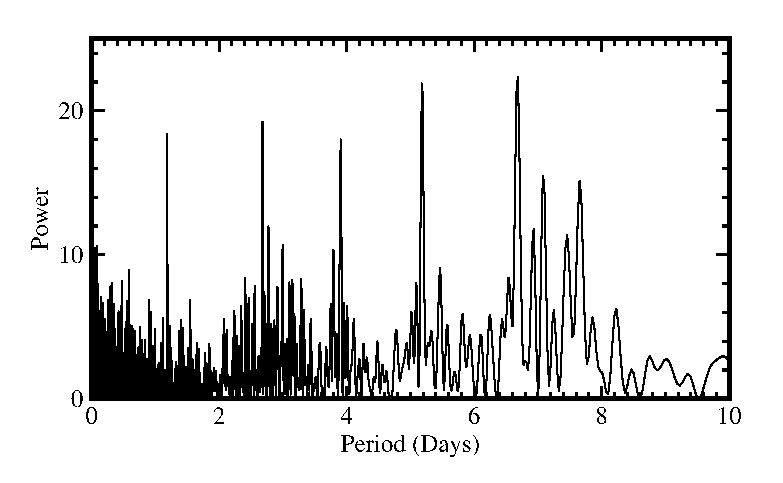
\includegraphics[width=7cm]{LS.eps}
%   \caption{Lomb-Scargle periodogram of the PDC lightcurve, with the
%     transits masked out. The lightcurve is rotationally modulated with
%   a period of 1.19 days.}
%   \label{fig:LS}
% \end{figure}

\section{Orbit obliquity from lightcurve asymmetry}
\label{sec:transit-light-curve}

\subsection{Lightcurve model}
\label{sec:lightcurve-model}

\begin{figure}
  \centering
  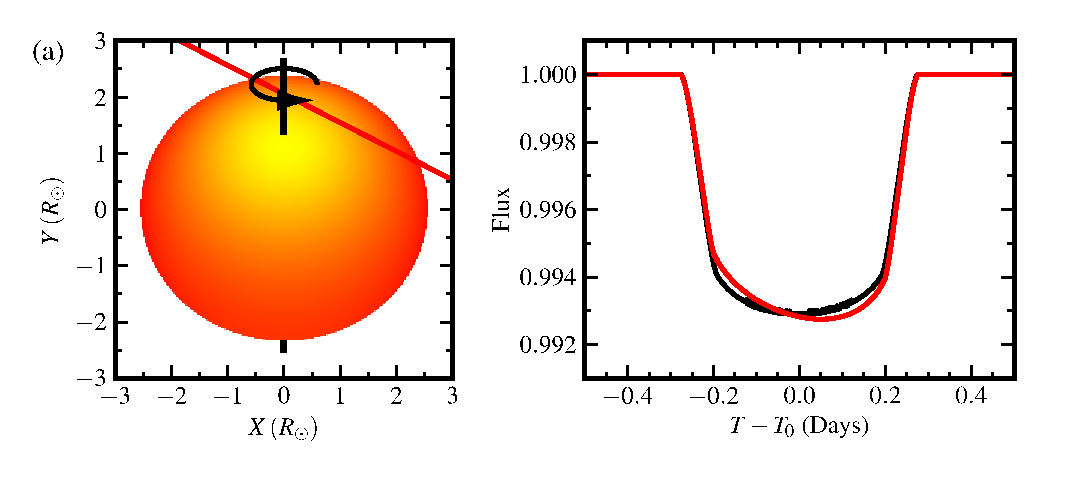
\includegraphics[width=9cm]{obliq_model.eps}
  \caption{f=0.2,beta=1.0,phi=0. Model using koi-368 system
    parameters (inc, rsum, rratio etc). 0, 45, 90 degree obliquity.}
  \label{fig:obliqmodel}
\end{figure}

\subsection{System parameter fitting}
\label{sec:model-fitting}

The transit lightcurve is modelled using the
\citet{Nelson1972} model, implemented in an adaption of the
JKTEBOP code \citep{Proper1981,Southworth2004}. The
relevant free parameters are orbital period $P$, transit centre $T_0$,
normalised radius sum $R_\star+R_p / a$, radius ratio $R_p/R_\star$,
line of sight inclination $i$. Quadratic limb darkening coefficients,
$c_1$ and $c_2$, 
are fitted for in an initial minimisation routine, with initial
estimates taken from \citet{Sing2010}, then held fixed for subsequent analyses. Jump
parameters for the stellar oblation correction include the planet
orbit obliquity $\lambda$, stellar oblation $f$. The projection angle
between the stellar rotation axis and line of sight $i_\text{rot}$ is
fixed for an initial analysis, then set free to explore the potential
degeneracies. The gravity darkening exponent $\beta$ is set to be
fixed at 0.25 [cite], but also allowed free in subsequent analysis to
explore degeneracies. A flux offset for each transit event is calculated and
removed at each iteration, and is not included in the fit
parameters. For Kepler long cadence data, the model is modified by a
30 minute boxcar smooth. The best fit parameters and the posterior
probability distribution is explored via a Markov chain Monte Carlo
(MCMC) analysis, using the \emph{emcee} MCMC ensemble sampler
\citep{ForemanMackey2012}. The likelihood function is given by
$\exp(-\Delta\chi^2/2)$. For each transit, we scale the flux errors such
that the reduced $\chi^2$ is at unity. This allows for errors other
than photon noise to be taken into account.

Figure~\ref{fig:lightcurve} plots the phase folded transit lightcurve of
KOI-368.01 and the best fit spherical and oblate models. The best fit
spherical host star model cannot explain the significant in-transit
asymmetry observed. The best fit parameters are presented in Table~\ref{tab:params}.

The posterior probability distributions for relevant parameters
are plotted in Figure~\ref{fig:posterior}. We find a weak inverse dependency
between $\lambda$ and $\beta$, and a positive dependency between
$\lambda$ and $R_p/R_\star$.

%%% Include parameter table
\begin{deluxetable*}{lrrr}
\tablewidth{0pc}
\tabletypesize{\scriptsize}
\tablecaption{KOI-368 System properties
\label{tab:params}}
\tablehead{
\multicolumn{1}{c}{Parameter} & 
\multicolumn{1}{c}{Spherical Model} &
\multicolumn{1}{c}{Limited Oblate Model} &
\multicolumn{1}{c}{Full Oblate Model} \\
}\startdata
\multicolumn{2}{l}{\textbf{Stellar parameters}}\\ 
$T_\text{eff}$ & $9200\pm500$ & - & -\\
$\log g$ & $4.1\pm0.5$ & - & -\\
$\text{[Fe/H]}$ & $0.0\pm0.5$ & - & -\\
$v \sin i_\text{rot}$ & $100 \pm 10$ & - & -\\
\\
\multicolumn{2}{l}{\textbf{Lightcurve fitting parameters \tablenotemark{1}}} \\ 
Period (Days) & $110.3216229_{-7}^{+3}$& $110.321615_{-6}^{+2}$ & $110.321613_{-7}^{+1}$ \\ 
$T_0$ $(\text{BJD}-2454000)$ & $1030.36382_{-3}^{+2}$& $1030.36407_{-9}^{+6}$ & $1030.36440_{-1}^{+3}$ \\ 
$(R_p+R_\star)/a$ & $0.02101_{-3}^{+1}$& $0.02078_{-5}^{+6}$ & $0.02103_{-2}^{+3}$ \\ 
$Rp/R_\star$ & $0.08401_{-5}^{+4}$ & $0.0866_{-2}^{+1}$ & $0.0854_{-1}^{+1}$ \\
$i$ & $89.209_{-1}^{+2}$ & $89.229_{-4}^{+3}$ & $89.209_{-2}^{+2}$ \\
$f$ & - & $0.064_{-6}^{+3}$ & $0.038_{-2}^{+2}$ \\
$\lambda$ & - & $67_{-7}^{+6}$ & $52_{-7}^{+5}$ \\
$\beta$ & - &- & $0.24_{-3}^{+2}$ \\
$i_\text{rot}$ & - & -  & $25_{-10}^{+4}$ \\
\\
\multicolumn{2}{l}{\textbf{Derived parameters}}\\ 

\enddata
\tablenotetext{1}{Uncertainties quoted are for the last significant figure}
\end{deluxetable*}

\begin{figure}[h!]
  \centering
  \includegraphics[width=9cm]{lightcurve.eps}
  \caption{Top: Phase folded transit lightcurve of KOI-368.01. Long
    cadence observations are plotted in black, short cadence in
    yellow. The best fit transit model for a spherical host star is
    plotted in blue, oblate host star in red. These two models are
    indistinguishable at this scale. Middle: Data residual to the
    spherical host star transit model. The long cadence data are
    plotted in full as gray dots. Long cadence data binned to 1 hour
    intervals are plotted in black, binned short cadence residuals in yellow. Bottom:
    Data residual to the oblate host star transit model.}
  \label{fig:lightcurve}
\end{figure}

\begin{figure*}[h!]
  \centering
  \includegraphics[width=12cm]{posterior.eps}
  \caption{Posterior probability distributions showing the correlation
  between the orbit obliquity $\lambda$ and stellar oblation $f$,
  radius ratio $R_p/R_\star$, gravity darkening exponent $\beta$, sky
  projected angle of the stellar rotation axis $i_\text{rot}$. The
  contours mark the 1 and 2$\sigma$ confidence regions. White contours
mark the distribution for the MCMC analysis with $\beta$ and
$i_\text{rot}$ fixed, the red contours show the distribution with
$\beta$ and $i_\text{rot}$ set free.}
  \label{fig:posterior}
\end{figure*}

\subsection{Asymmetry from eccentricity}
\label{sec:asymm-from-eccentr}

A highly eccentric orbit can also cause asymmetric distortions to the
transit lightcurve. An eccentric orbit distorts the lightcurve by
changing the planet's velocity through the transit. We explore the
possibility that the lightcurve distortions observed for KOI-368.01
are due to an eccentric instead of an oblique orbit.

Following \citet{Barnes2007}, we can constrain the change in velocity
$(\Delta v = v_\text{out} - v_\text{in})$ by measuring the difference
in the duration of ingress and egress $(\Delta t)$,
\begin{align}
  \Delta t &= \frac{R_p}{v_\text{out} \cos\left(\sin^{-1} b \right)} -
  \frac{R_p}{v_\text{in} \cos\left(\sin^{-1} b \right)} \\
  \Delta v &\approx v^2 \frac{\Delta t \cos \left( \sin^{-1} b \right)}{R_p}
\end{align}
where $b = a \cos i/R_\star = 0.7$ is the transit impact parameter, and $v =
\sqrt{G M_\star / a} = 43.3\,\text{kms}^{-1}$. Using
the short cadence data, we measure ingress and egress durations to be
equal to within errors of 0.7 minutes, constraining the maximum
possible change in velocity to be $\Delta v <
0.5\,\text{kms}^{-1}$. Figure~\ref{fig:eccmode} plots the difference between such an
eccentric orbit lightcurve and its best fit circular orbit
lightcurve. The maximum in-transit distortions are $10
\times$ smaller than that for the oblique orbit model. The maximum
distortions during ingress and egress are $5\times$ smaller than that
for the oblique orbit model, and are not consistent in shape to that
observed for KOI-368.01. The lightcurve distortions for KOI-368.01
therefore cannot be explained by an eccentric orbit.

\begin{figure}[h!]
  \centering
  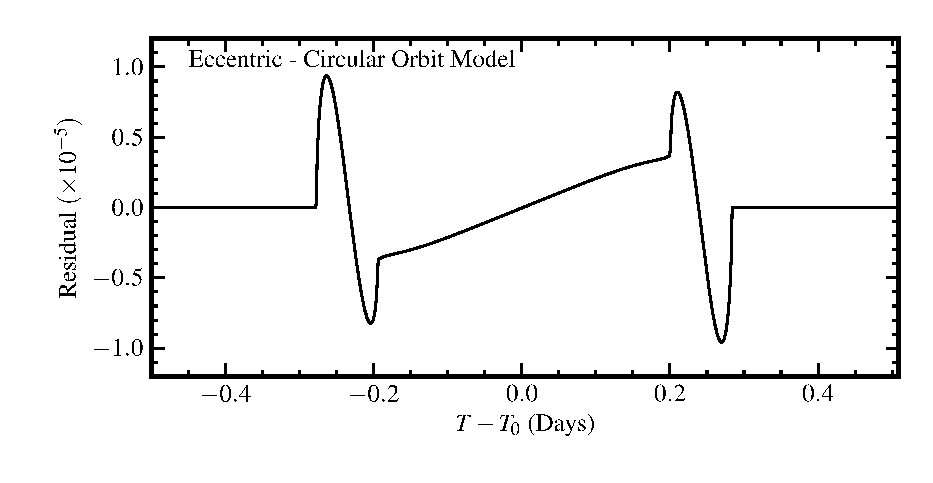
\includegraphics[width=7cm]{ecc_model.eps}
  \caption{The maximum lightcurve distortions due to a
    eccentric orbit for KOI-368.01 are plotted as residuals to its
    best fit circular orbit model. The maximum velocity change is
    determined by measuring the difference in the ingress and egress
    duration. Eccentricity cannot explain the observe lightcurve
    asymmetry (Figure~\ref{fig:lightcurve}, middle panel).}
  \label{fig:eccmodel}
\end{figure}


% \citet{Barnes2007} calculated such an effect for the
% favourablely eccentric hot-Jupiter HD 147506b to be $\sim10^{-6}$ on
% the lightcurve, an order of magnitude
% smaller than the distortions observed for KOI-368.01. We present the
% following arguments that the observed lightcurve distortions for
% KOI-368.01 are not due to an eccentric orbit. 1) KOI-368.01 has an orbital period 20 times longer than that of HD
% 147506b, and will need an orbital eccentricity of $>0.96$ to
% experience the same maximum change in velocity over a transit as that
% HD 147506b. 2) This maximum change occurs directly before or after
% periastron. Such an orbit will cause a transit wiht duration shorter
% than that of a circular orbit. This is contradicted by the measured
% transit duration of KOI-368.01. 3) An eccentric orbit results in
% asymmetric timescales for ingress and egress, which is not observed.


\section{Nature of the companion}
\label{sec:nature-companion}

[Blends in images]

A stellar mass M-dwarf companion will cause a secondary eclipse in the
lightcurve. We mask out the primary transit and remove large scale
variations the Kepler long cadence lightcurve using a cosine filter
with minimum width of 1 day. We perform a grid
search for a secondary eclipse, in the phase space between 0.05 and
0.95, using the \citet{Mandel2002} eclipse model. We can rule out the
presence of any secondary eclipse event with depth
$>10^{-5}$. Assuming the system is not a blend, we can constrain the
temperature of the orbiting companion to be $< 2500\,\text{K}$, and
must be of sub-stellar nature.

\subsection{System eccentricity}
\label{sec:system-eccentricity}

The system eccentricity can be constrained by comparing the measured
transit duration $(t_\text{obs}=13.2\,\text{hours})$ against that expected for a circular
orbit \citep[e.g.][]{Barnes2007,Burke2008,Kane2012}. Adopting host star
parameters of $M_\star = 2.2\,M_\odot$ and $R_\star = 2.1\,R_\odot$
[cite/ref], the expected circular orbit transit duration is
$t_\text{circ} =9.8\,\text{hours}$. Following \citet{Burke2008}, we
solve for $e$ in
\begin{equation}
  \label{eq:ecc}
  \frac{t_\text{obs}}{t_\text{circ}} = \frac{\sqrt{1-e^2}}{1+e \cos(\omega-\pi/2)}\,,
\end{equation}
and find $0.3 < e < 1$, depending on the argument of periastron $\omega$. This range is highly
dependent on the assumed host star parameters, which are not well
measured. For a host star with 30\% smaller radius, we find the
eccentricity is constrained to be $>0.9$ for all $\omega$. In the case
of a host star 30\% larger than quoted, we can place no constraints on
eccentricity. 


\section{Discussion}
\label{sec:discussion}

\begin{figure}[h]
  \centering
  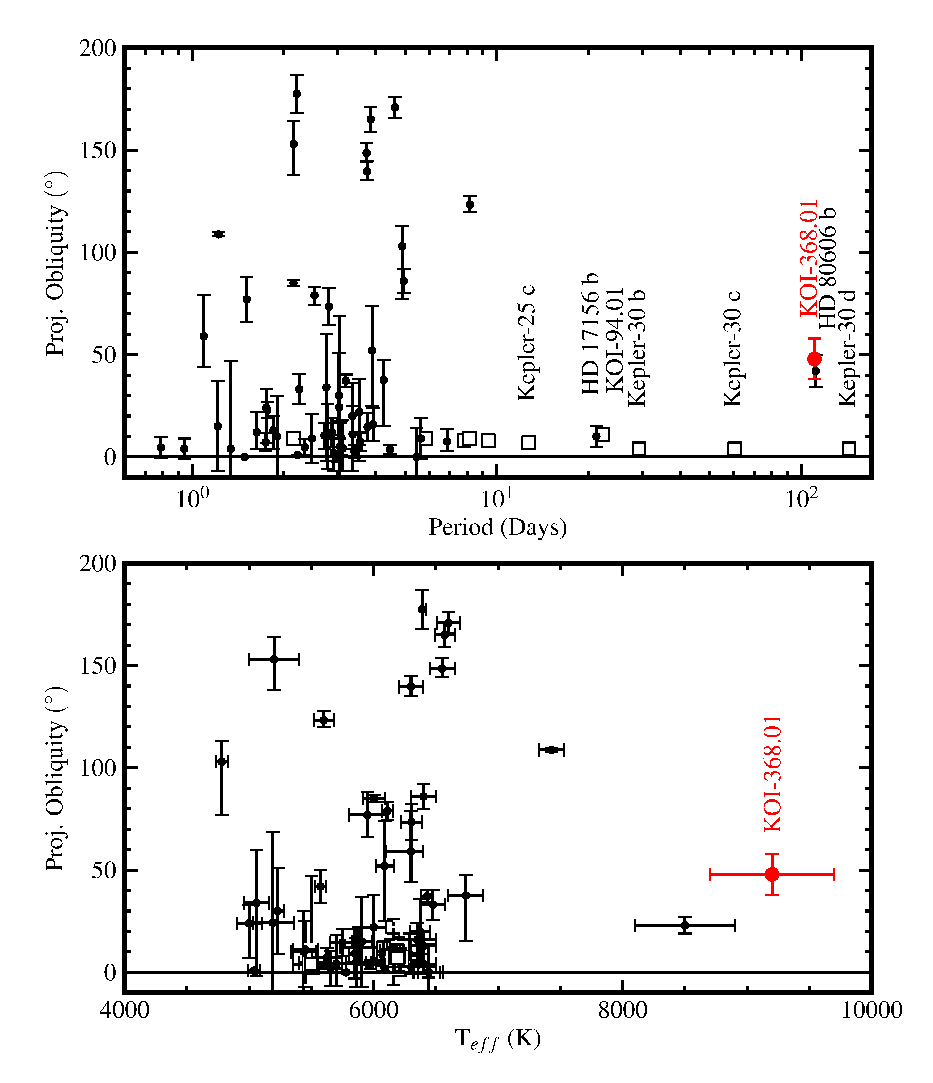
\includegraphics[width=9cm]{period_obliq.eps}
  \caption{caption}
  \label{fig:periodobliq}
\end{figure}

\bibliographystyle{apj}
\bibliography{mybibfile}

\end{document}
